% !TeX root = ../main.tex
\section{Uniform FBG modelling through discretised reflections}
\label{sec:FBG_discretised}
%
To overcome the limitations of convolution-based models and the absence of analytical ECM analyses, we seek a representation of FBG feedback that links directly to physical parameters while preserving the mathematically tractable delay–differential structure of the LK equations.
One promising route is to approximate the distributed reflection process directly in the time domain through discretised reflections.
Although most approaches in the literature begin with the spectral response of the grating, the reflection spectrum can also be modelled by approximating the grating as a sequence of discrete layers, each contributing a reflection and transmission event \cite{poladian2000simple, ghiringhelli2002time, feced2002efficient, skaar2001synthesis}.
This construction amounts to a discretised version of the impulse response $\tilde{\rho}(t)$ that would otherwise be obtained from $\rho(\omega)$ by an inverse Fourier transform.
By considering all optical paths that re-emerge from the FBG after a delay of $\tau_k$, the impulse response can be written as a weighted sum of delta functions,
%
\begin{equation}
    \label{eq:dicretised_impulse}
    \tilde{\rho}(t) = \sum_{k=0}^N h_r(k)\, \text{Dirac}(t-\tau-\tau_k)
\end{equation}
%
which we refer to as the discretised impulse response.
Physically, $h_r(k)$ encodes the effective amplitude of all paths contributing to the delayed signal emerging after a time delay $\tau_k$ as illustrated in Figure~\ref{fig:discretised_FBG}(a).
For non-uniform gratings, the average refractive index varies along the structure, requiring distinct refractive indices $n_i$ and corresponding transmission and reflection coefficients $t_{i,i+1}$ and $r_{i,i+1}$ to be computed for each layer.
This approach has been shown to recover the spectral response $\rho(\omega)$ with high accuracy \cite{ghiringhelli2002time}.
Here, however, we focus on the simpler case of uniform FBGs, where the average index is constant along the grating, so that all layers are identical.
This simplification yields a particularly transparent formulation of the feedback term $F(t)$ in terms of the coefficients $h_r(k)$, without requiring explicit reference to the full spectral response.
%
\par
%
We will show in the following that an approximate model for this discretised-reflection framework retains the analytic tractability of the Lorentzian FOF model discussed in section~\ref{subsec:FOF}, while also faithfully reproducing the reflection spectrum of uniform FBGs across a broad frequency range.
This combination of accuracy and simplicity opens the way to both closed-form equations for cavity modes, efficient numerical integration, and advanced numerical methods such as continuation.
%
%
\subsection{Uniform FBG discretised reflection model derivation}
\label{subsec:FBG_discretised_derivation}
%
\begin{figure}[!t]
    \centering
    
    \begin{overpic}[width=0.95\linewidth]{Images/discretised_reflections.pdf}
        \put(-1,60){(a)}
    \end{overpic}\\[0.5em]
    \begin{overpic}[width=0.95\linewidth]{Images/single_reflection_tk.pdf}
        \put(-1,60){(b)}
    \end{overpic}
    
    \caption{(a) Illustration of the first six layers in the slab decomposition of a uniform FBG, showing transmission and reflection coefficients between adjacent layers ($j=i+1$).
    (b) Illustration of the contribution to the reflected field arising solely from reflection at the $k^{\text{th}}$ layer, corresponding to the $k^{\text{th}}$ delayed signal.}
    
    \label{fig:discretised_FBG}
\end{figure}
%
\begin{figure}[!t]
    \centering
    
    \hspace{0.04cm}
    \begin{overpic}[width=\linewidth]{Images/R_tau_discretised_accuracy.pdf}
        \put(-4,93){(a)}
        \put(-4,48){(b)}
    \end{overpic}

    \caption{A comparison between the exact (solid lines) total reflection \eqref{eq:R_exact} and discretised (dashed lines) total reflection \eqref{eq:R_approx} is shown in (a), and the exact effective delay \eqref{eq:tau_exact} and discretised delay expectation \eqref{eq:tau_approx} is shown in (b) as functions of the normalised refractive index variation $\dn$ for varying $N \in [10,100,1000,10000]$.}

    \label{fig:R_approximations}
\end{figure}
%
We model the reflection response of a uniform FBG as arising from partial reflections at evenly spaced boundaries across $N$ layers of the grating.
The grating has a uniform average refractive index $\neff$, while each boundary introduces the same transmission coefficient $t$ and reflection coefficient $r$, determined by the normalised refractive index variation $\dn \equiv \dnbar/\neff$.
Further, the constant $\neff$ ensures that the round-trip time $\dt$ is constant across all layers so that $\tau_k = k \, \dt$.
For tractability, we consider only the dominant propagation paths that undergo a single reflection at the $(k-1)^\text{th}$ layer.
A contribution from such a path re-emerges from the grating after a time delay of $k\,\dt$, as sketched in Figure~\ref{fig:discretised_FBG}(b).
In this way, the discretised model mirrors the idea of an impulse response composed of delayed replicas of the input field, but expressed in terms of individual layer reflections.
%
\par
%
For the discretised formulation to be meaningful, it must reproduce the essential characteristics of a uniform FBG, most importantly the total reflectivity $R$, while linking the effective coefficients $r$ and $t$ to the physical parameters of the grating.
The exact reflectivity of a uniform FBG at its Bragg frequency, given by \eqref{eq:rmax}, can be written as
%
\begin{equation}
\label{eq:R_exact}
R_\text{exact} = \tanh{\left(\frac{\pi}{2}\frac{N \, \dn}{1+\dn} \right)}.
\end{equation}
%
A key observation is that this expression is very well approximated by the simpler form
%
\begin{equation}
\label{eq:R_approx}
R_\text{approx} = 1 - \left(1 - \dn \right)^{2N},
\end{equation}
%
as shown in Figure~\ref{fig:R_approximations}(a), where both forms are plotted as a function of $\dn$ for different $N$.
The close agreement confirms that the discretised model reproduces the correct scaling of reflectivity with both modulation depth and grating length.
To connect this approximation to a reflection model, we represent the signal emerging from the front facet after a time delay $k \, \dt$ as having passed through $k-1$ transmissive layers before being reflected at the $k^\text{th}$ layer, with no further attenuation thereafter.
The corresponding contribution is
%
\begin{equation}
\label{eq:hr1}
h_r(k) = t^{k-1} r,
\end{equation}
%
where $t$ and $r$ denote the effective transmission and reflection coefficients.
To ensure consistency with \eqref{eq:R_approx}, these coefficients must reproduce the total reflectivity when all delayed reflections are summed.
Rewriting \eqref{eq:R_approx} as a geometric series,
%
\begin{align*}
R_\text{approx} &= 1 - (1-\dn)^2 + (1-\dn)^2 - \dots \\
&\hspace{1em} - (1-\dn)^{2N-2} + (1-\dn)^{2N-2} - (1-\dn)^{2N} \\
&= \left( 1-(1-\dn)^2 \right)\left( 1 + (1-\dn)^2 + \dots + (1-\dn)^{2N-2} \right) \\
&= (1-(1-\dn)^2)\sum_{k=1}^{N} \left((1-\dn)^2\right)^{k-1},
\end{align*}
%
we arrive at an expression that is exactly reproduced by \eqref{eq:hr1} if we define
%
\begin{align}
\label{eq:tr}
t &\equiv (1-\dn)^2, \\
r &\equiv 1-(1-\dn)^2.
\end{align}
%
\par
%
Because FBGs act as distributed reflectors, it is not sufficient for the discretised model to match only the total reflectivity; it should also capture the effective delay of the structure, which represents how the reflected energy is distributed in time across multiple paths.
This can be tested by comparing the average delay predicted by the discrete reflections, $E[\tau_\text{FBG}]$, with the effective delay $\tau_{eff}$ derived directly from the exact reflection spectrum \cite{barmenkov2006effective}.
The effective time delay can be written in terms of the layer round-trip time $\dt = 2 \Lambda \neff/c$ as
%
\begin{equation}
    \label{eq:tau_exact}
    \tau_{eff} = \frac{R_\text{exact} \dt}{\pi \, \dn}.
\end{equation}
%
The expected delay of the discretised reflections $E[\tau_\text{FBG}]$ is calculated as the weighted average of the delays of all the reflected signals, where the weights are the amplitudes of the reflected signals.
Mathematically,
%
\begin{equation*}
    E[\tau_\text{FBG}] = \frac{r \sum_{k=1}^{N} t^{k-1} (k-1)\dt}{r \sum_{k=1}^{N} t^{k-1}}.
\end{equation*}
%
The sum in the denominator is simply the sum of a geometric sequence, having a closed form
%
\begin{equation*}
    \sum_{k=1}^{N} t^{k-1} = \frac{1-t^N}{1-t}.
\end{equation*}
%
The sum in the numerator can be evaluated efficiently by noting that it can be written in terms of a derivative w.r.t. $t$ of the numerator.
That is,
%
\begin{equation*}
    \sum_{k=1}^{N} t^{k-1} (k-1) = t \, \frac{\partial}{\partial t} \sum_{k=1}^{N} t^{k-1} = \frac{t(1-t^N)}{(1-t)^2} - \frac{N t^N}{1-t}.
\end{equation*}
%
The effective delay then simplifies to
%
\begin{equation}
    \label{eq:tau_approx}
    E[\tau_\text{FBG}] = \dt\left[ \frac{t}{1-t} - \frac{N t^N}{1-t^N} \right].
\end{equation}
%
\par
%
Figure~\ref{fig:R_approximations}(b) compares the effective delay $\tau_{eff}$ with the expected delay $E[\tau_\text{FBG}]$ of the discretised model, plotted as a function of $\dn$ for different $N$.
The comparison shows that the discretised model reproduces the effective delay with high accuracy, matching closely at small $\dn$ and diverging only gradually at larger values.
Although the accuracy of delay and reflectivity vary differently with $\dn$, the model reproduces both with sufficient consistency to remain reliable across the full parameter range.
%
\par
%
A key property of the coefficients in \eqref{eq:tr} is that they satisfy $r+t=1$, resembling the familiar balance between reflection and transmission.
Unlike true Fresnel coefficients, however, these are effective coefficients: they subsume the cumulative effect of multiple internal transmissions and reflections into a single pair of parameters.
In doing so, they preserve the correct scaling of reflectivity with $\dn$ and $N$ while providing a compact, physically transparent description that is straightforward to use in dynamical models such as the LK equations.
%
\begin{equation}
    \label{eq:discretised_impulse_full}
    \tilde{\rho}(t) = (1-t)\sum_{k=0}^{N-1} t^k \, \delta(t-\tau-k\dt)\, e^{-i k \wB \dt},
\end{equation}
%
where each term corresponds to a contribution that has traversed $k$ transmissive layers, been reflected once, and accumulated an additional phase $e^{-i k \wB \dt}$ from propagation through the grating.
Since the LK equations are defined relative to the free-running laser frequency (so that $\wZ=0$), the parameter $\wB$ naturally enters as the detuning of the grating's Bragg frequency.
This highlights that the FBG acts as a weighted superposition of delayed, phase-shifted replicas of the input field.
We remark that if backward transmission were explicitly included, alternative but mathematically consistent definitions of $r$ and $t$ could be derived, though the present choice yields cleaner expressions for the analysis that follows.
%
\par
%
With this foundation, the feedback term $F(t)$ follows directly as the convolution of the field with \eqref{eq:discretised_impulse_full}, consistent with earlier convolution-based formulations \cite{skenderas2024impact,skenderas2021feedback,li2012distributed,li2015chaotic,li2020stable}:
%
\begin{align*}
F(t) &= e^{-i C_p} E(t) \otimes \tilde{\rho}(t) \\
&\approx r e^{-i C_p} \sum_{k=0}^{N-1} t^k E(t) \otimes \delta(t-\tau-k\,\dt) e^{-i k \wB \dt} \\
F(t) &\approx (1-t) e^{-i C_p} \sum_{k=0}^{N-1} t^k E(t-\tau-k\,\dt) e^{-i k \wB \dt}.
\end{align*}
%
\par
%
Taken together, these results establish the discretised-reflection formulation as a reliable and practical approximation to FBG feedback.
Crucially, it preserves the analytic tractability of the LK system while embedding essential features of grating physics, thereby enabling both efficient time-domain simulations and deeper analytical exploration of cavity modes.
The central parameter $t$, which enters the LK equations, is determined directly from the target reflectivity via \eqref{eq:R_approx}:
%
\begin{equation}
\label{eq:discretised_t}
t = \big(1-R\big)^{1/N},
\end{equation}
%
providing a transparent connection between physical grating design and the discrete-feedback model.
This link ensures that the formulation is not only computationally convenient but also grounded in experimentally tunable parameters, making it a robust foundation for the analyses that follow.
%
\par
%
With both reflectivity and effective delay validated, the discretised model can now be embedded directly into the LK equations, which take the form
%
\begin{equation}
\label{eq:LK_discretised}
    \begin{aligned}
        \frac{d E}{d t} = (1 &+i \a) N(t) E(t) + \\
                        &\quad \eta (1-t) e^{-i C_p} \sum_{k=0}^{N-1} t^k E(t-\tau-k\, \dt) e^{-i k \wB \dt} \\
        T \frac{d N}{d t} &= P-N(t)-(1+2 N(t))|E(t)|^2.
    \end{aligned}
\end{equation}
%
Unlike convolution-based models, this formulation reduces the feedback to a finite sum of discrete delays, preserving the DDE structure for ECM analysis and continuation, while also providing a platform to explore the spectral properties of the system through its mode structure.
%
%
\subsection{EGM modes of the discretised reflection model}
\label{subsec:EGM_discretised}
%
A natural first step in assessing any feedback model is the calculation of its cavity modes, since these steady-state solutions provide the `backbone' of the system and reveal how the feedback reshapes the laser’s mode structure.
In the COF and FOF cases, mode calculations (ECMs and EFMs, respectively) have been central to validating both the physical realism and the analytical tractability of the models.
For the discretised FBG reflection model, the corresponding external grating modes (EGMs) serve the same purpose: they provide a direct spectral interpretation of the formulation, constitute the first point of comparison with the known reflection properties of uniform FBGs, and act as benchmarks for demonstrating that the model captures not only physical but also spectral characteristics of FBG feedback.
Beyond this role in validation, EGMs also structure much of the system’s dynamics and stability \cite{rottschafer2007ecm}, and once stable solutions are identified they can be systematically continued in parameters using specialised DDE continuation software such as \texttt{DDE-BifTool}.
%
\par
%
The EGMs take the form $(E(t), N(t)) = (E_s e^{i\w_s t}, N_s)$ with $E_s, \w_s, N_s \in \mathbb{R}$, corresponding to a laser field oscillating at a shifted frequency $\w_s$ with constant amplitude $E_s$ and inversion $N_s$.
Physically, $\w_s$ represents the detuning of the locked field from the solitary laser frequency $\w_0$.
Substituting this ansatz into \eqref{eq:LK_discretised} yields an implicit equation for the allowed EGM frequencies.
To this end, we first separate the resulting complex equation into its real and imaginary parts by expanding the exponentials, giving
%
\begin{align*}
    i \w_s = (1+i \a) N_s &+ \eta (1-t) \big(\cos{(\phi_\text{E})} -i\sin{(\phi_\text{E})}  \big) \times \\ 
                        &\left( \sum_{k=0}^{N-1} t^k \cos{(k\phi_\text{F})} - i \sum_{k=0}^{N-1} t^k \sin{(k\phi_\text{F})} \right)
\end{align*}
%
where $\phi_\text{F} = \dt(\wB + \w_s), \, \phi_\text{E} = C_p+\tau \w_s$ are the phases accumulated in the FBG and EC, respectively.
To evaluate the sums in closed form, we use the standard trigonometric series identities
%
\begin{align*}
    \sum_{k=0}^{N-1} &t^k \cos{(k\phi_\text{F})} = \\
    &   \frac{1 - t \cos{(\phi_\text{F})} - t^N \cos{(N\phi_\text{F})} + t^{N+1} \cos{((N-1)\phi_\text{F})}}{1 - 2t \cos{(\phi_\text{F})} + t^2} \\
    \sum_{k=0}^{N-1} &t^k \sin{(k\phi_\text{F})} = \\
    &\quad \quad \frac{t \sin{(\phi_\text{F})} - t^N \sin{(N\phi_\text{F})} + t^{N+1} \sin{((N-1)\phi_\text{F})}}{1 - 2t \cos{(\phi_\text{F})} + t^2}
\end{align*}
%
an implicit equation for the EGM frequencies $\w_s$ can be derived,
%
\begin{gather*}
    \begin{aligned}
\w_s = \frac{\eta (1-t) \sqrt{1 + \a^2}}{1 - 2 t  \cos{(\phi_\text{F})} + t^2} \times \\
&&\hspace{-6em} \Big[- &\sin{(\phi_\text{E} + \arctan\a)} \\
&&\hspace{-6em}      +  t&\sin{(\phi_\text{E} + \arctan\a - \phi_\text{F})} \\
&&\hspace{-6em}      + t^N&\sin{(\phi_\text{E} + \arctan\a + N \phi_\text{F})}   \\
&&\hspace{-6em}      -  t^{N+1}&\sin{(\phi_\text{E} + \arctan\a + (N-1) \phi_\text{F})}
\Big].
    \end{aligned}
\end{gather*}
%
After algebraic simplification, the right-hand side can be expressed as a single sine term, leading to
%
\begin{equation}
    \label{eq:discretised_ws}
    \w_s = -\eta (1-t) \sqrt{\a^2+1}\frac{S_N}{S} \sin{\left( \phi_\text{E}+\arctan\a + \Phi - \Phi_N  \right)}
\end{equation}
%
where
%
\begin{align}
    S &= \sqrt{1 - 2 t \cos{(\phi_\text{F})} + t^2}
    \\
    S_N &= \sqrt{1 - 2 t^N \cos{(N\phi_\text{F})} + t^{2N}}
    \\
    \Phi &= \arctan{\left( \frac{t \sin{(\phi_\text{F})}}{1 - t \cos{(\phi_\text{F})}} \right)} 
    \\
    \Phi_N &= \arctan{\left( \frac{t^N \sin{(N\phi_\text{F})}}{1 - t^N \cos{(N\phi_\text{F})}} \right)}.
\end{align}
%
We remark that in the plane mirror limit, the front face of the FBG would reflect all incoming light, that is $ t = 0 \implies S = S_N = 1, \, \Phi = \Phi_N = 0$, yielding 
%
\begin{equation*}
    \w_s = - \eta \sqrt{\a^2+1} \sin{(C_p + \w_s \tau + \arctan\a )}
\end{equation*}
%
which is precisely the well studied implicit ECM equation for the canonical COF case, validating the consistency of the derived equations \cite{rottschafer2007ecm}.
Given the solutions for $\w_s$, one can calculate $N_s$ and $E_s$ through
%
\begin{equation}
    N_s = -\eta (1-t) \frac{S_N}{S} \cos{\left( \phi_\text{E} + \Phi - \Phi_N \right)}  
\end{equation}
%
\begin{equation}
    E_s = \sqrt{\frac{P - N_s}{1 + 2 N_s}}
\end{equation}
%
The envelope of $f$, defined as $f_\text{env}(\w_s)$, is obtained by taking the extreme values of the sine term in \eqref{eq:discretised_ws}, i.e., setting it to $\pm 1$.
%
\begin{equation}
    \label{eq:discretised_ws_envelope}
    f_\text{env}(\w_s) = \mp \eta (1-t) \sqrt{\a^2+1}\frac{S_N}{S}
\end{equation}
%
Moreover, by substituting the CW ansatz back into \eqref{eq:LK_discretised}, one obtains an explicit expression for $N_s(\w_s)$, given by
%
\begin{gather}
    \label{eq:discretised_Ns_curve}
    \begin{aligned}
        \hspace{-0.5em}N_s(\w_s) = &\frac{\a \w_s}{1+\a^2} \pm \\
                    &\frac{1}{1+\a^2}\sqrt{-\w_s^2 + (1+\a^2) \left(\eta (1-t) \frac{S_N}{S} \right)^2}.
    \end{aligned}
\end{gather}
%
Finally, while the grating’s reflectivity and detuning are controlled through $\eta$ (or $R$) and $\wB$, respectively, the number of layers $N$ provides an additional design parameter, directly setting the FBG bandwidth $\wz$ via \eqref{eq:wz} and \eqref{eq:R_approx}.
%
\begin{equation}
    \label{eq:wztoN}
    \wz = \w_\text{max} \sqrt{\left( \frac{1 - (1 - R)^\frac{1}{2N}}{2} \right)^2 + \frac{1}{N^2}}
\end{equation}
%
\begin{figure}[!t]
    \centering 
    
    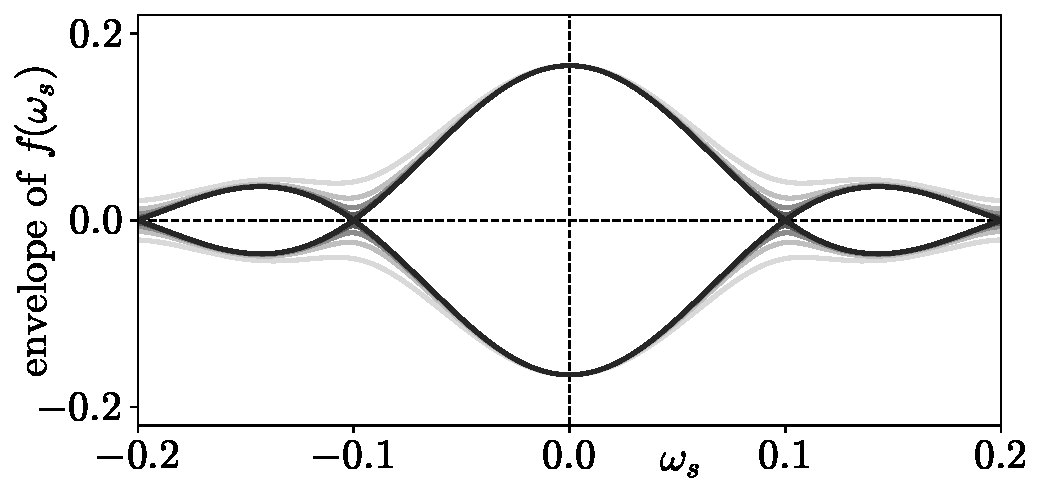
\includegraphics[width=\linewidth]{Images/discretised_EGM_envelope_variations.pdf}   
    
    \caption{Variation in the shape of the envelope $f_\text{env}(\w_s)$ for $R \in [0.01, 0.2, 0.4, 0.6, 0.8]$ while keeping the effective feedback rate $\eta R$ constant.}
    
    \label{fig:discretised_EGM_envelope_variations}
\end{figure}
%
\begin{figure}[!t]
    \centering
    \hspace{1em}
    \begin{overpic}[width=0.9\linewidth]{Images/Low_N_gratings.pdf}
        \put(-5,54){(a)}
    \end{overpic} \\
    \vspace{1em}
    \begin{overpic}[width=\linewidth]{Images/discretised_EGM_varyN.pdf}
        \put(0,82){(b)}
        \put(0,40){(c)}
    \end{overpic}  \\
    \vspace{1em}
    \makebox[\linewidth][c]{%
    \hspace{1em}%
    \begin{overpic}[width=0.99\linewidth]{Images/discretised_EGM_wideview.pdf}
        \put(-1,42){(d)}
    \end{overpic}%
    }
    \caption{(a) Illustrations of gratings with equal length but different layer numbers $N$.
    (b), (c) Equivalence in EGM structure between different grating numbers $N \in [10, 22500]$ by keeping $N\dt$ constant, each providing near identical reflection zero locations $\wB \pm n\wz, \; n \in \mathbb{N}$.
    EGM frequencies $\w_s$ are intersections of $f(\w_s)$ (blue curve) and $g(\w_s)$ (green curve) in (a), while the envelope $f_\text{env}$, consisting of two curves is in black.
    The EGM solutions and their curve in the $(\w_s, N_s)$-plane are shown in (b).
    The red dots correspond to a discrete set of EGMs, where modes are indicated with circles while antimodes are indicates by squares.
    The black curve connecting the the set of EGMs is given by \eqref{eq:discretised_Ns_curve}.
    (d) EGM solutions over a wide frequency range $\w_s \in [-20\wz, 20\wz]$.
    In panels (b)–(d), results for $N=10$ are plotted in lighter shades, while results for $N=22500$ are plotted in darker shades.
    }

    \label{fig:discretised_EGM_varyN}
\end{figure}
%
\begin{figure*}[!t]
    \flushleft
    \hspace{1em}
    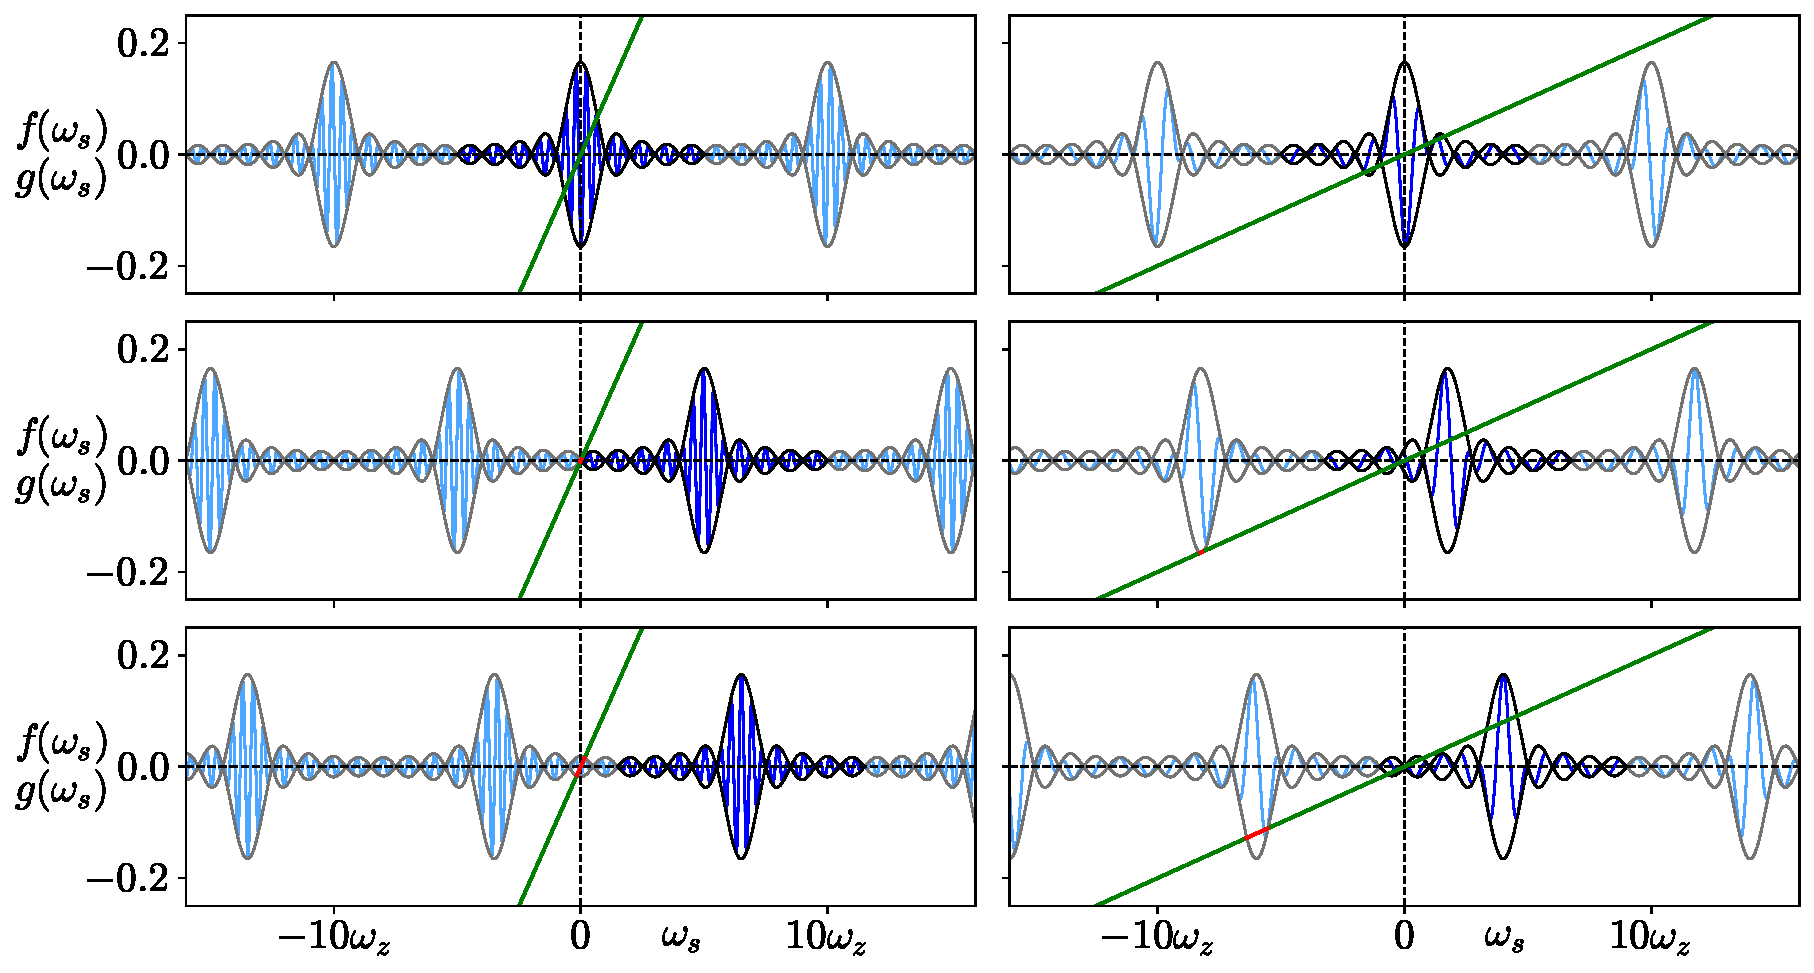
\includegraphics[width=0.87\linewidth]{Images/discretised_EGM_minimumN.pdf}
    
    \caption{EGM solutions for varying detuning $\wB$ with $\wz=0.1$ (left) and $\wz=0.02$ (right) and $N=10$ in both cases.
    Valid region solution regions correspding to the frequency range $\wB \pm 5 \wz$ are plotted with opaque lines while the entire frequency region is plotted with semi transparent lines.}
    
    \label{fig:discretised_EGM_minimumN}
\end{figure*}
%
\par
%
At this point, the EGM equations allow us to directly visualise the spectral structure predicted by the discretised reflection model.
In particular, the solution envelope $f_\text{env}(\w_s)$ provides a direct analogue of the FBG reflection spectrum, just as the envelope in the FOF case recovers a Lorentzian profile \cite{green2006mode}, while the envelope in the COF case being flat (and thus frequency indepedent) \cite{rottschafer2007ecm}.
This makes it a natural diagnostic for selecting the effective grating parameters $(R, N, \dt)$.
To anchor the discussion, we fix the laser and EC parameters to the canonical values $\tau = 121, \a = 3.5, \eta R = 0.0455, C_p = 0, T = 550, P = 0.186$ \cite{heil2003delay,krauskopf2004dynamics}, and prescribe a grating bandwidth $\wz = 0.1$ with detuning $\wB=0$.
For 1550 nm light, this choice of $\wz$ corresponds to $N \approx 22500$ layers (see Appendix~\ref{app:LK_nondim} for details).
%
\par
%
We first examine how the envelope changes with reflectivity $R$ while keeping the product $\eta R$ fixed.
As shown in Figure~\ref{fig:discretised_EGM_envelope_variations}, well-resolved transmission zeros at $\w_s = \wB \pm n\wz$ emerge only when $R$ is small.
This motivates adopting the practically relevant limit $R\ll1$, in which $\eta$ is rescaled so that the effective feedback rate $\eta_\text{eff} \equiv \eta R$ remains fixed.
In this regime, \eqref{eq:wztoN} simplifies to
%
\begin{equation}
\label{eq:wz_approx}
\wz \approx \frac{2\pi}{N \dt},
\end{equation}
%
so that the bandwidth is controlled entirely by the product $N\dt$, or equivalently, by the physical grating length $L = N \dt c/\neff$.
%
\par
%
This simplification provides a powerful degree of freedom: $N$ can be reduced substantially without altering the envelope spectrum, provided $N\dt$ is kept constant.
Figure~\ref{fig:discretised_EGM_varyN}(b) illustrates this invariance, showing near-identical envelopes for gratings with $N$ ranging from $10$ to $22500$ once $N\dt$ is matched.
Physically, this reflects the intuition that short gratings behave as broadband reflectors, while longer gratings act as narrowband filters.
The ability to tune $N$ while preserving the spectral response means the model can be kept numerically tractable for continuation and integration.
%
\par
%
Beyond the excellent agreement in the envelopes $f_\text{env}(\w_s)$ for drastically different $N$, Figure~\ref{fig:discretised_EGM_varyN}(a) additionally illustrates the strong agreement between the curves $f(\w_s)$ and $g(\w_s)$, defined as as the left- and right-handside of \eqref{eq:discretised_ws}, respectively.
In the standard way, EGM solutions visualised in the $(\w_s, N_s)$-plane in (b) are found numerically by the intersections $f(\w_s)$ and $g(\w_s)$ shown in (a) and mirror the excellent agreement already demonstrated with the solution envelopes.
In this case, the EGMs lie within the main lobe on the closed curve given by \eqref{eq:discretised_Ns_curve} with modes (stable EGMs) indicated by circles lying on the lower portion of the curve and anti-modes (unstable EGMs) indicated by squares lying on the upper portion of the curve.
It is noted that agreement in the solutions degrades for EGMs with larger frequency detunings $\w_s$, although the agreement is still reasonable for practical purposes.
We therefore may select a layer number $N$ that is low enough to be amenable to standard numerical analyses such as continuation without encountering significant computational difficulties.
%
\par
%
The main practical consequence of working with a reduced grating number $N$ is that only a limited number of side lobes are reproduced accurately.
Figure~\ref{fig:discretised_EGM_varyN}(d) illustrates this by plotting the curves $f(\w_s)$ and $f_\text{env}(\w_s)$ over $\w_s \in [-20\wz,20\wz]$ for $N=10$ and $N=22500$ with $N\dt$ fixed.
When $N=10$, the envelope repeats after every $10\wz$, so that only five side lobes are physically meaningful before the spectrum develops unphysical repetitions.
By contrast, the $N=22500$ case reproduces the correct extended sequence of side lobes expected from a uniform FBG.
This highlights the need to choose $N$ small enough to keep the model tractable, but large enough to capture all features relevant to the parameter ranges under study.
%
\par
%
Figure~\ref{fig:discretised_EGM_minimumN} shows two specific artefacts that arise if $N$ is taken too small, allowing a lower bound on $N$ to be derived.
The first is a detuning-induced loss of validity: as $\wB$ increases, the valid spectral window of width $\pm 5\wz$ can shift away from $\w_s=0$, and beyond this range the repeated envelope begins to grow again, which is unphysical.
This can be avoided by requiring $N > 2|\wB|_{\max}/\w_{z,\min}$.
The second artefact is the appearance of spurious intersections when repeated main lobes cross the line $f(\w_s)=\w_s$, creating artificial EGM branches.
The first repetitions of the main lobe occur at $\w_s = \pm N\wz + \wB$, while the envelope reaches extrema at $\pm \eta\sqrt{1+\a^2}$.
To prevent such intersections, one must ensure that $N\wz + |\wB| > \eta\sqrt{1+\a^2}$.
Taken together, these two requirements provide a practical lower bound for the grating number:
%
\begin{equation}
    \label{eq:Nmin}
    N_\text{min} =
    \begin{cases}
    \left\lceil \dfrac{2|\wB|_{\max}}{\w_{z,\min}} \right\rceil, \; |\wB|_{\max} > \eta_{\max}\sqrt{1+\a_{\max}^2}, \\[2ex]
    \left\lceil \dfrac{|\wB|_{\max} + \eta_{\max}\sqrt{1+\a_{\max}^2}}{\w_{z,\min}} \right\rceil, \; \text{otherwise}.
    \end{cases}
\end{equation}
%
With these conditions satisfied, the discretised model remains spectrally faithful while retaining the low dimensionality needed for efficient continuation and simulation.
%
\par
%
Taken together, these observations show that the EGM envelope both recovers the expected reflection spectrum and guides the principled choice of grating parameters.
Small $R$ ensures accurate reflection zeros, the product $N\dt$ fixes the bandwidth, and the lower bound in \eqref{eq:Nmin} guarantees physical side-lobe structure.
With these conditions, the discretised model remains both spectrally faithful and computationally manageable.